\part{Analysis}
\vspace{30pt}
\begin{center}
\textit{Well begun is half done}
\source{Aristotle}
\end{center}
\vspace{30pt}
In this section, we will attempt to give the reader insight into the rationale behind the decisions made in the course of the project, by reflecting on challenges and surprises uncovered by analysing the problem area. In other words, the section will try to explain \textit{why} the system has been designed as it has, why the process has been managed the way it has, and so on.

The section is structured by the various techniques and artefacts used in conducting the analysis. The primary topics covered in this section are:
\begin{itemize}
\item Business modelling
\item Requirements analysis
\item Data modelling
\item Architectural analysis
\end{itemize}
We begin the section by investigating and discussing the activities aimed at uncovering requirements for the system.
\section{Requirements Analysis}
Generally speaking, requirements can be divided into two categories; functional and non-functional. The functional requirements for the RentIt server are expressed by use-cases, that each encapsulate some functionality the system must posses in order to be a useful solution. The non-functional requirements are captured by the factor-tabel.
  These artefacts will serve as the basis for the discussion of the requirements in this section.
\subsection{Use Cases}
As mentioned, the use-cases capture the functional requirements of the system. The list of use cases was composed by examining the business model and identifying user goals associated with uploading, viewing and buying videos, creating user accounts and so on.

When writing use cases for the RentIt system, we noted that they could be grouped into three categories of usage:
\begin{itemize}
\item \textbf{User management}\\
Use cases concerning user profile creation, editing user profiles and authorizing users
\item \textbf{Video management}\\
Use cases concerning downloading, viewing and rating videos
\item \textbf{Transaction management}\\
Use cases concerning transactions between account balances and buying more RentIt credits.
\end{itemize}
In other words, the use cases reveal at least three major areas of responsibility within the required functionality of the system. These responsibilities imply a large scale organization of namespaces, by way of the GRASP principles.

In addition, the use cases provided some intuition about the control flow of some of the major operations of the system. Take for example user case no. 11, which describes paying for a video:\\

\textbf{A user wishes to pay for a video}
\begin{itemize}
	\item Precondition: The user has an active account with sufficient money deposited
	\item Postcondition: The user has the appropriate amount withdrawn from his 				account
	\item Postcondition: The user is granted access to the video
	\begin{enumerate}
		\item The user finds the video he wants to buy
		\item The user indicates that he wants to buy the video
		\item The user is granted access to the video
	\end{enumerate}
\end{itemize}

While short and simple, the pre- and postconditions as well as the steps involved in the use case, reveal a number responsibilities and changes in control flow to be considered. For example, the precondition indicates that each user has a balance associated with her account, to which deposits are made  in a separate use case (no. 9). Furthermore, the following responsibilities need to be delegated to appropriate branches of the system
\begin{itemize}
\item withdrawing money from the users account
\item granting users access to videos upon successful payment
\end{itemize}
This insight can be used as inspiration when designing the large scale organization of namespaces, and the control flow between these packages.

Moreover, the use cases proved an effective way of communicating ideas with the SMU group. By comparing our use cases with their use case model, it was possible to reconcile the two groups expectations to the semantic meaning of the different operations of the system. Take for example use case no. 4, dealing with purchasing videos:\\

\textbf{A user wants to see a video and downloads it to his computer}
\begin{itemize}
\item Precondition: User is logged in
\item Precondition: User has enough credits to pay the video
\item Postcondition: The video is saved on the users computer
\item Postcondition: The appropriate amount is subtracted from the users account
\begin{enumerate}
\item Available videos are presented to the user
\item The user selects the video he wants to see
\item The user is presented with options to rent and buy
\item The user selects buy
\item The user specifies where the file should be saved
\item The download begins
\end{enumerate}
\end{itemize}

This use case was utilized as the basis of a discussion between our own and the SMU group, about the semantic meaning of the term "buy", by the end of which it was decided that downloading a video constituted a buy, whereas renting would involve streaming the video, which is also expressed in the use case.

\subsection{Factor Table}
As opposed to the functional requirements, the non-functional requirements are not expressed by some functionality the system must offer, but rather some behaviour or quality the system must posses. These are captured by a factor table, as described in \textbf{Larman}. The list of factors the factor table consists of, was devised by using the FURPS+ mnemonic, and brainstorming on predictable requirements based on the business model. This facilitated a fruitful discussion on topics such as security, reliability and performance requirements of the system. The factor table can be found below:
\begin{center}
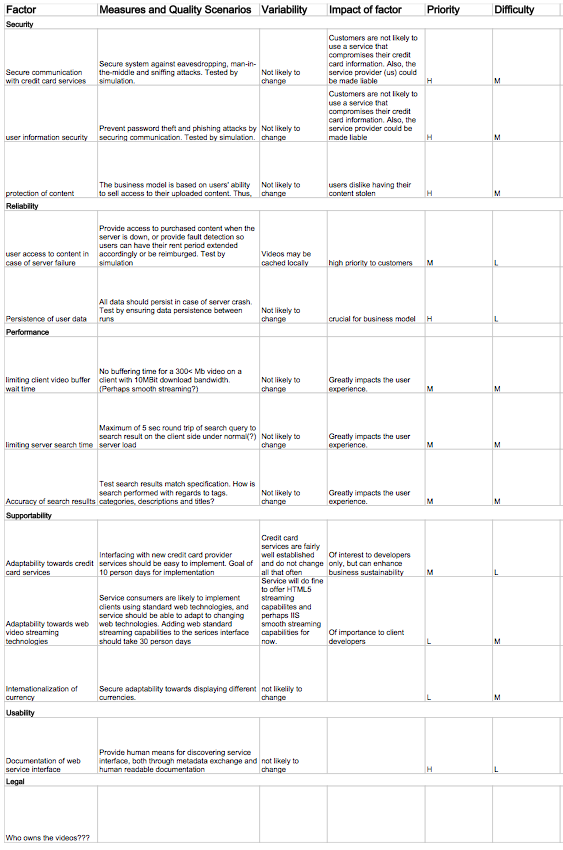
\includegraphics[scale=1.3]{FactorTable.png}
\end{center}
The 

Some of the usefulness of the factor table is its recording of quality scenarios, because it encouraged the group to reflect on the quantifying the requirement, as to make it testable. Realistically, it would not be possible to satisfactory implement and test all of the factors, but for the sake of exercise, the factor table was composed as if it was meant to be used in  real world situation. As a consequence of the limited timeframe of the project, we decided to limit the factors that we would \textit{actually} emphasize to:
\begin{itemize}
\item accuracy of search results
\item documentation of web service interface
\item persistence of user data
\end{itemize}

These factors were consensually understood as the most crucial and/or interesting requirements to pursue.

\section{Data Modelling}
Another major part of our problem analysis was devising a model of the data, partly in order to construct and refine a database design for persisting the necessary data, and in part to serve for inspiration for C\# classes.
This modelling was done using two artefacts, a domain to serve as a visual dictionary for objects and concepts in the problem domain, and an ER-diagram as an aid for reflecting on a useful database design. The main inspiration for these models were the use cases and the business model. These two artefacts serve the basis for discussions in this section.
\subsection{Domain Model}
The domain model was used to facilitate and document the results of a discussion of the problem domain. By modelling the objects and concepts in the problem domain, the project group came upon a number of questions, such as:
\begin{itemize}
\item 
\end{itemize}
\begin{center}
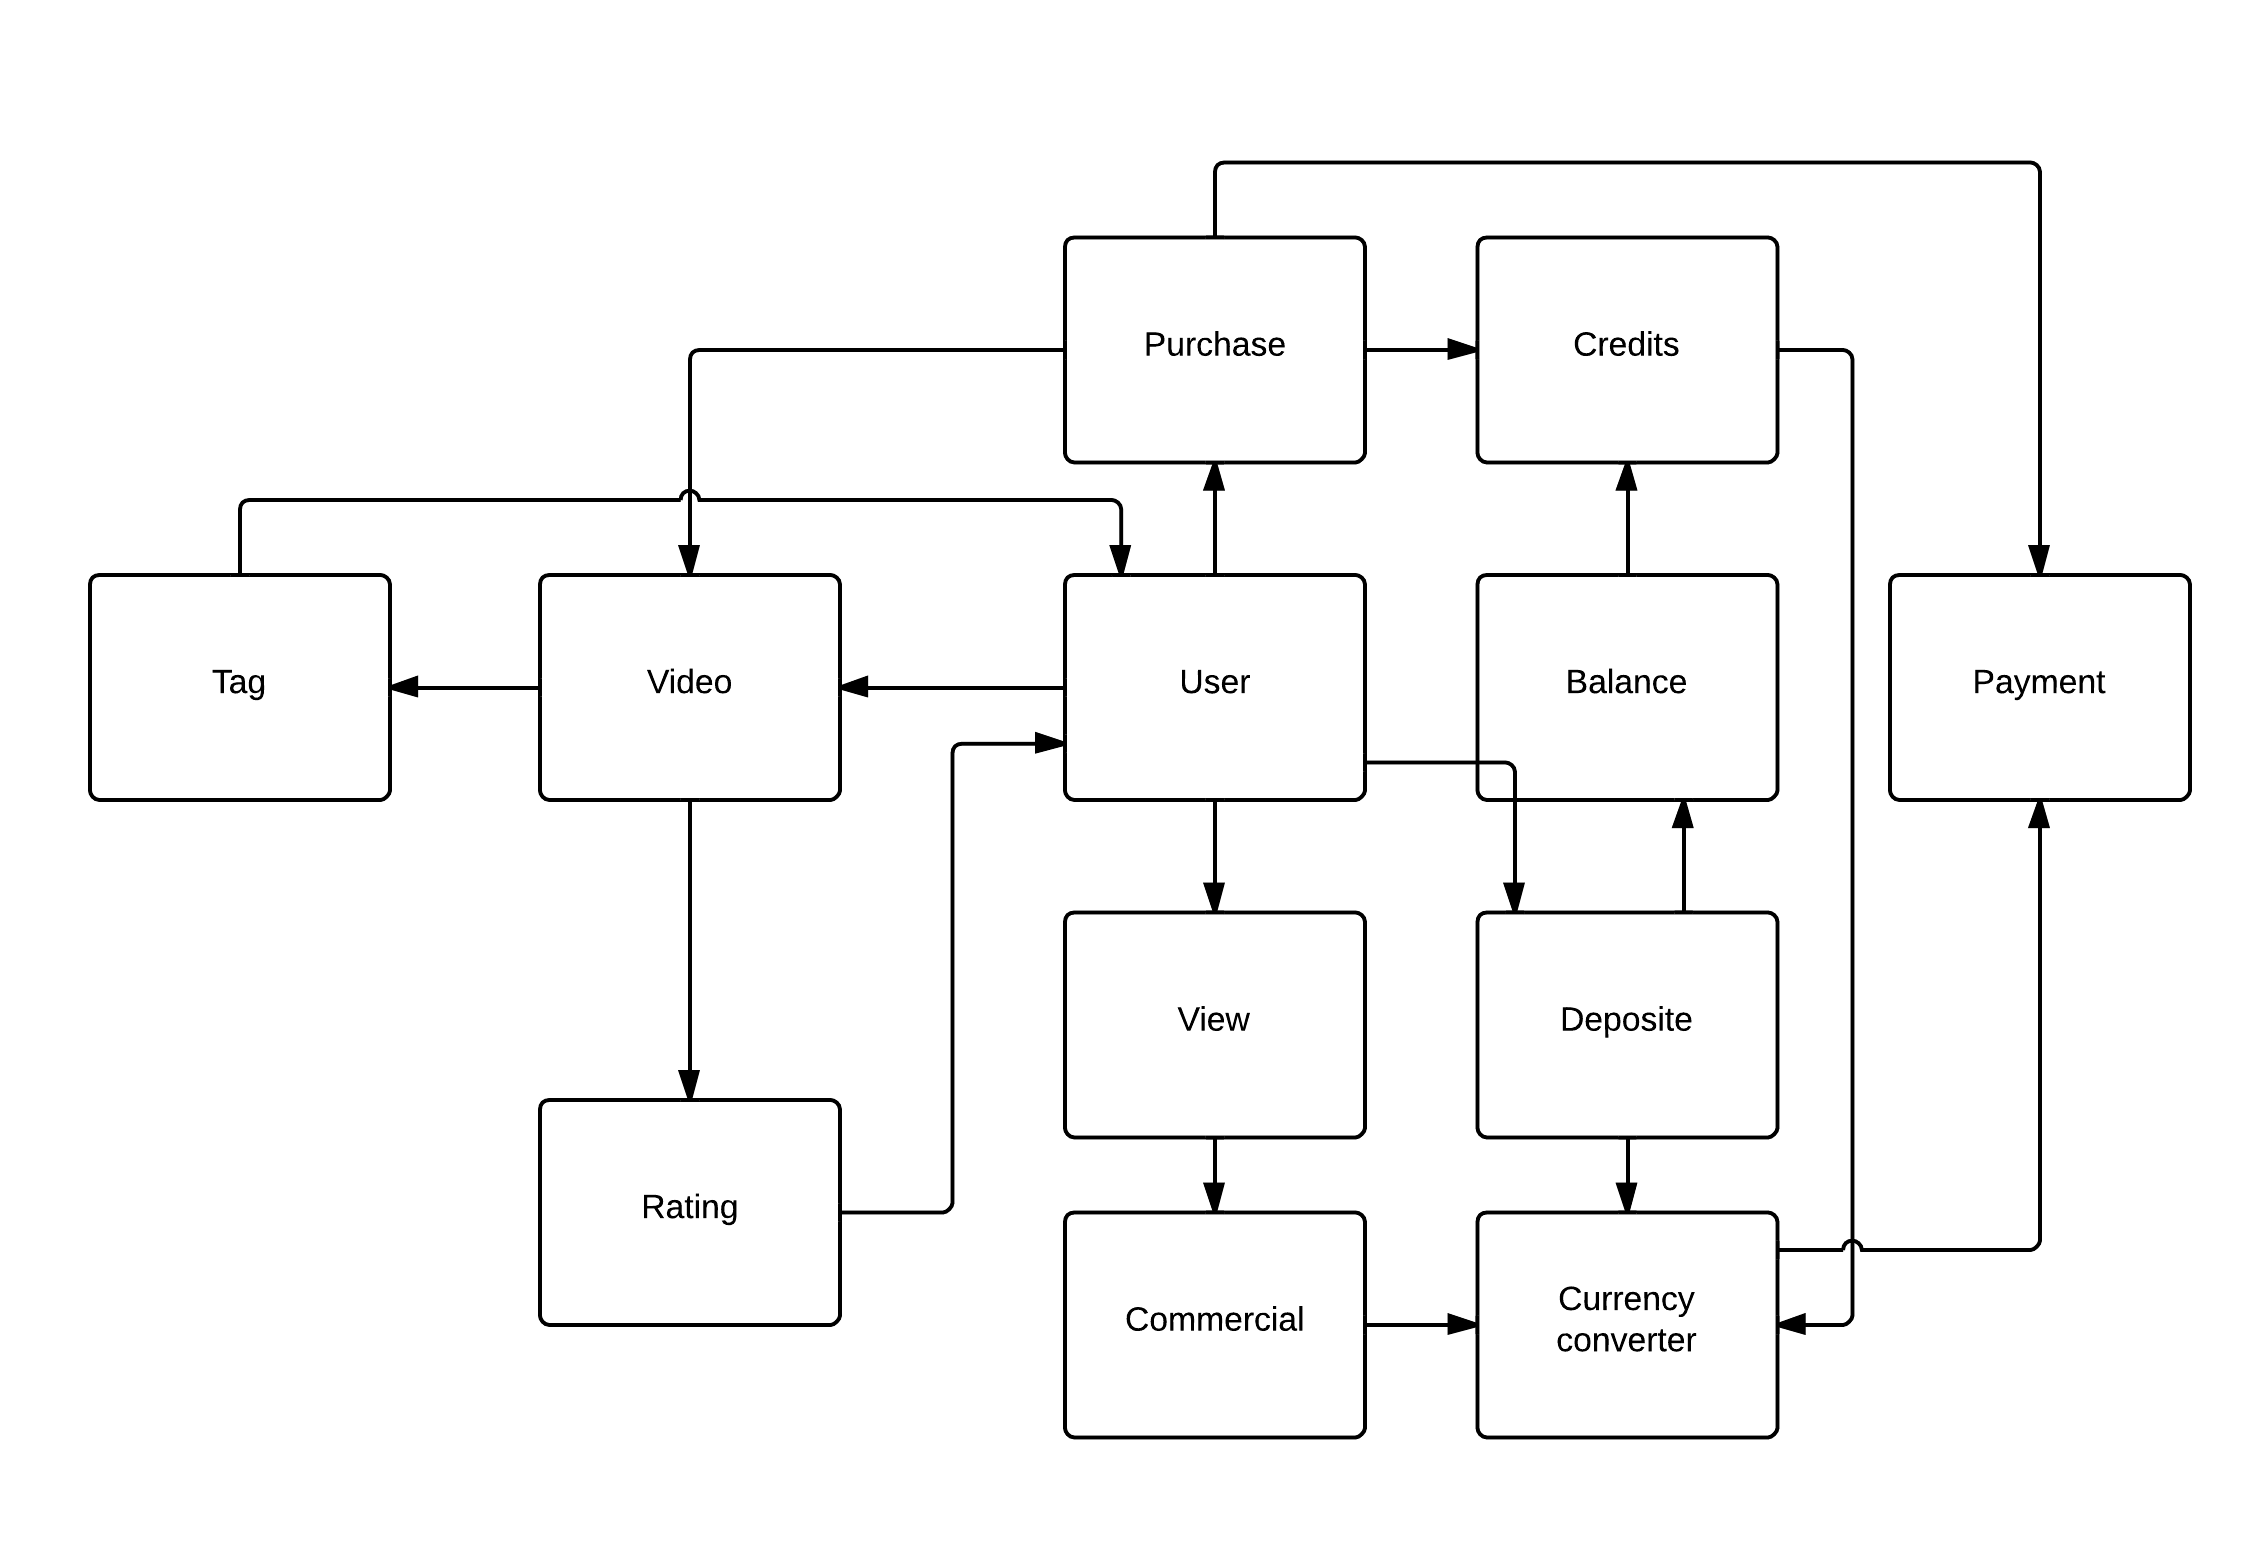
\includegraphics[scale=0.15]{DomainModel.png}
\end{center}

\subsection{ER-Diagram}
\begin{center}
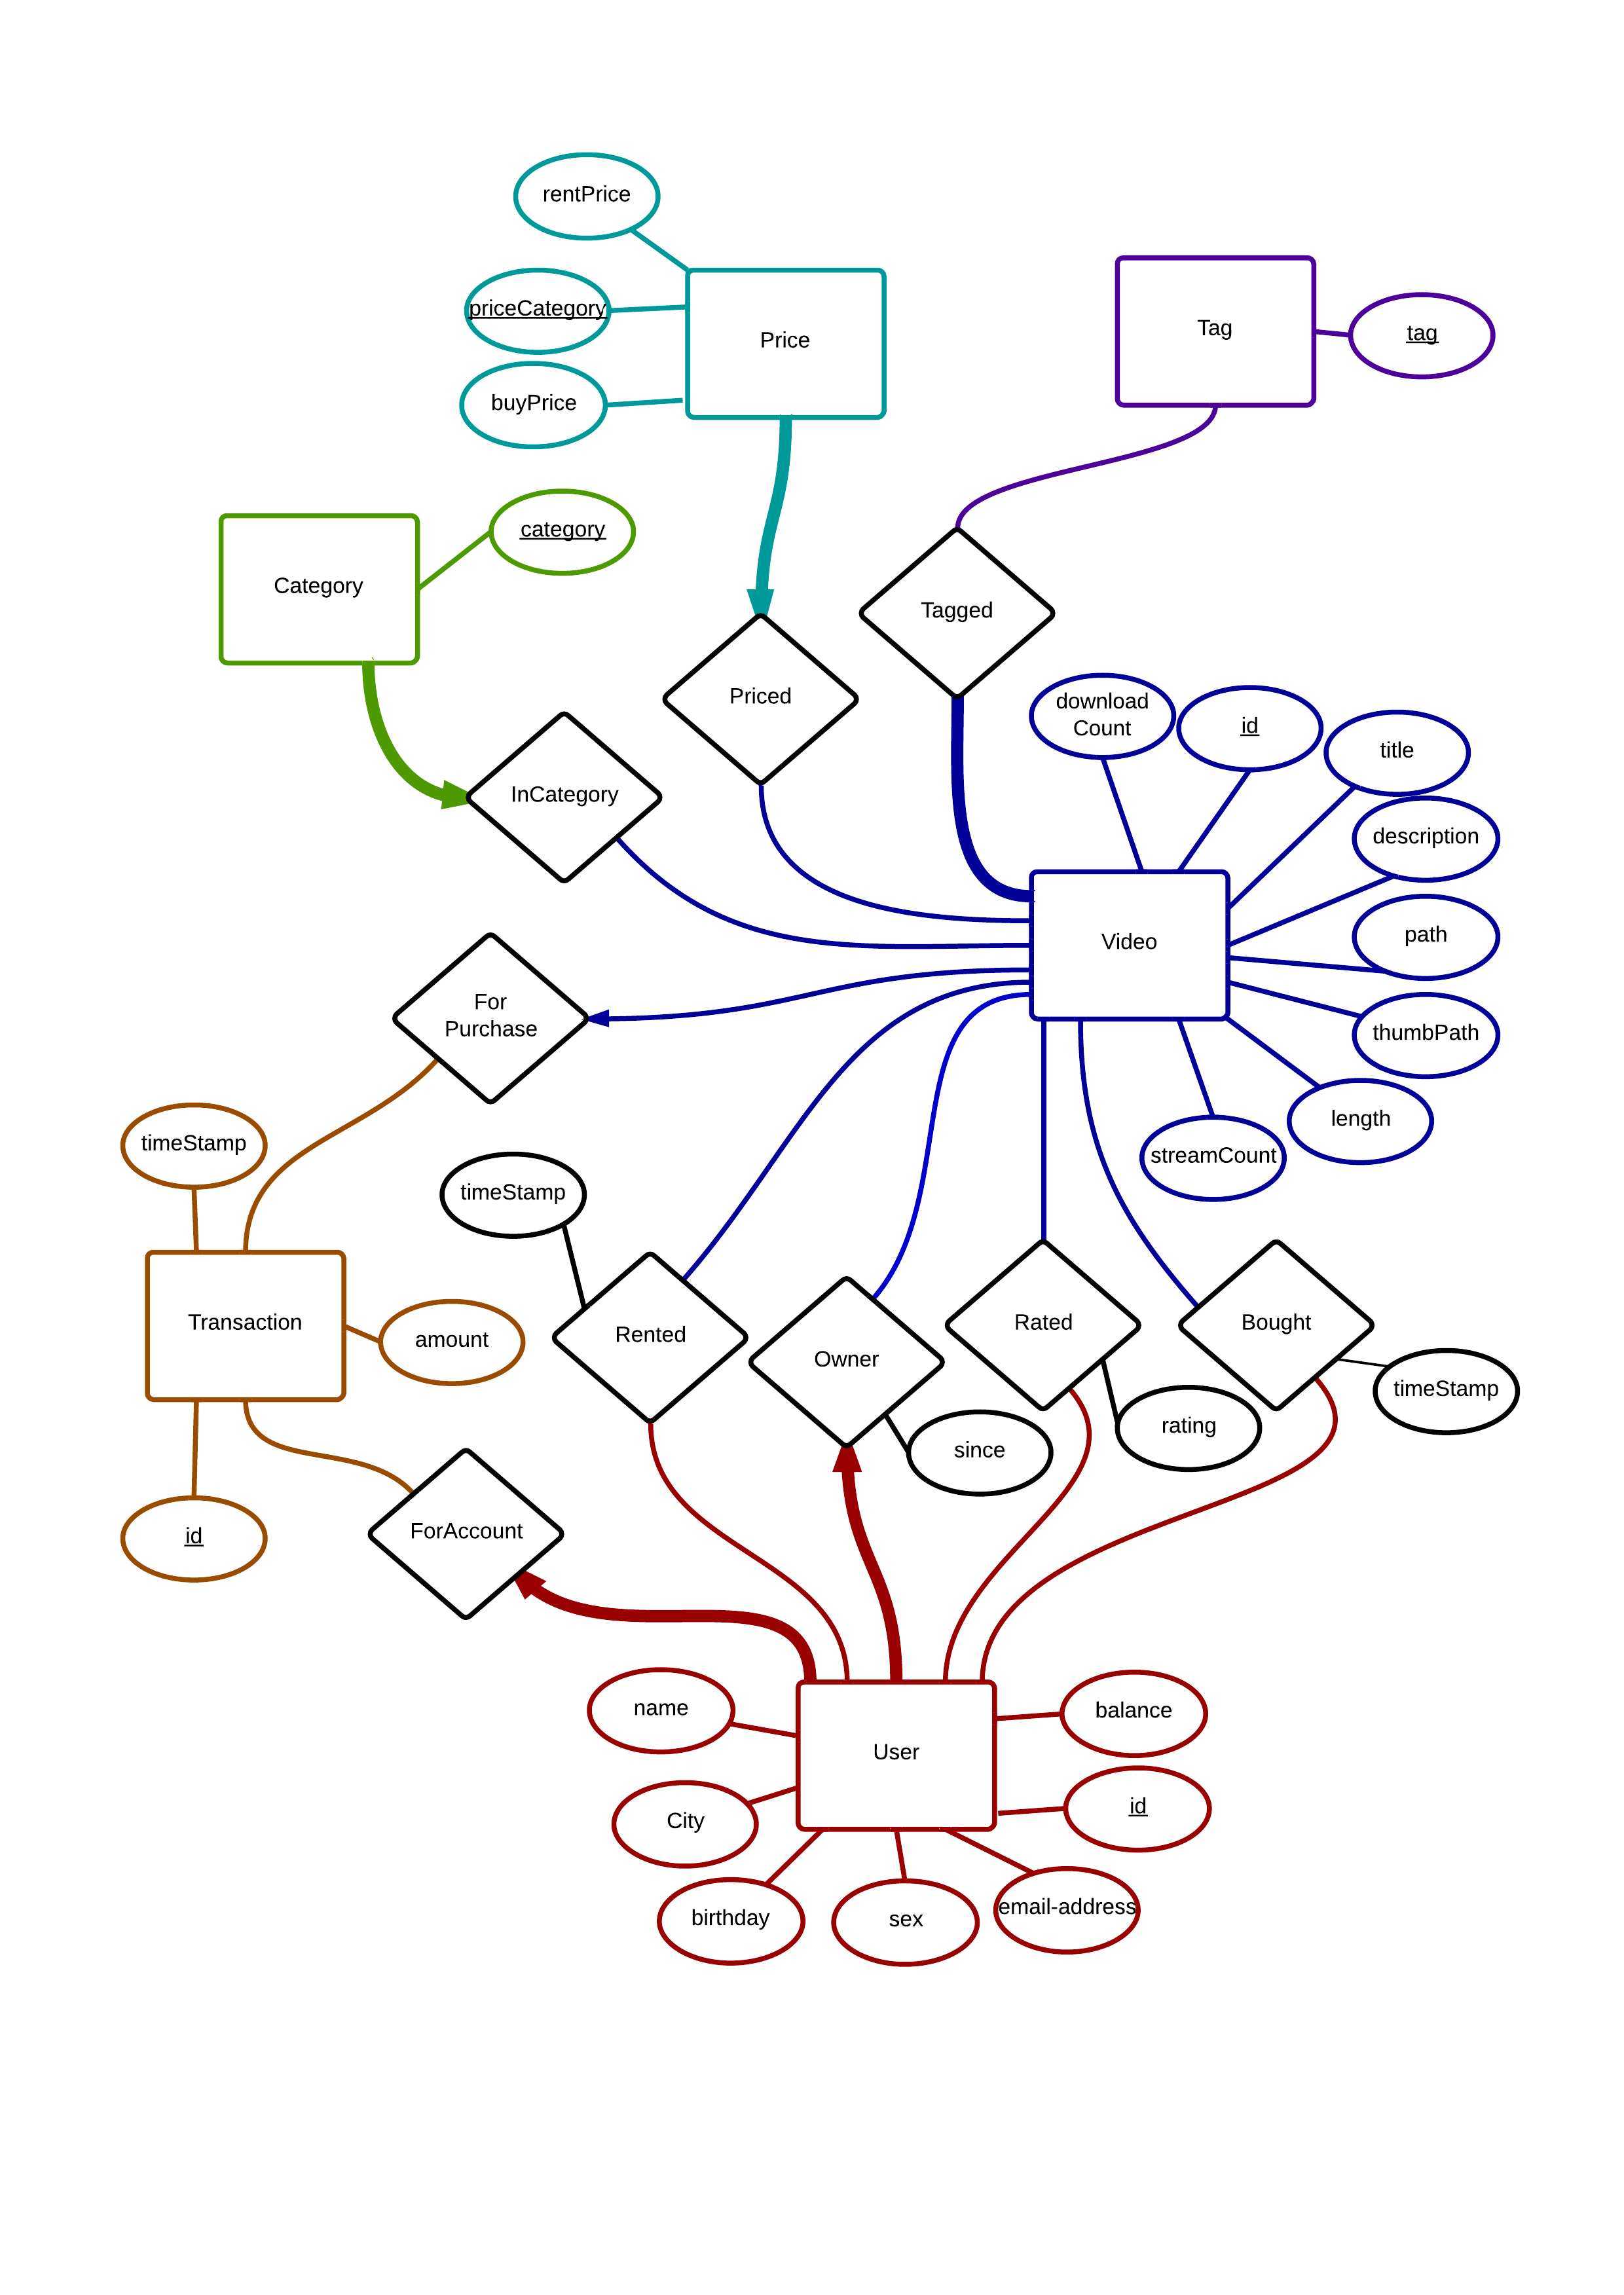
\includegraphics[scale=0.15]{ERDiagram.png}
\end{center}

\section{Architectural Analysis}
In this section
\subsection{Package Diagram}
\begin{center}
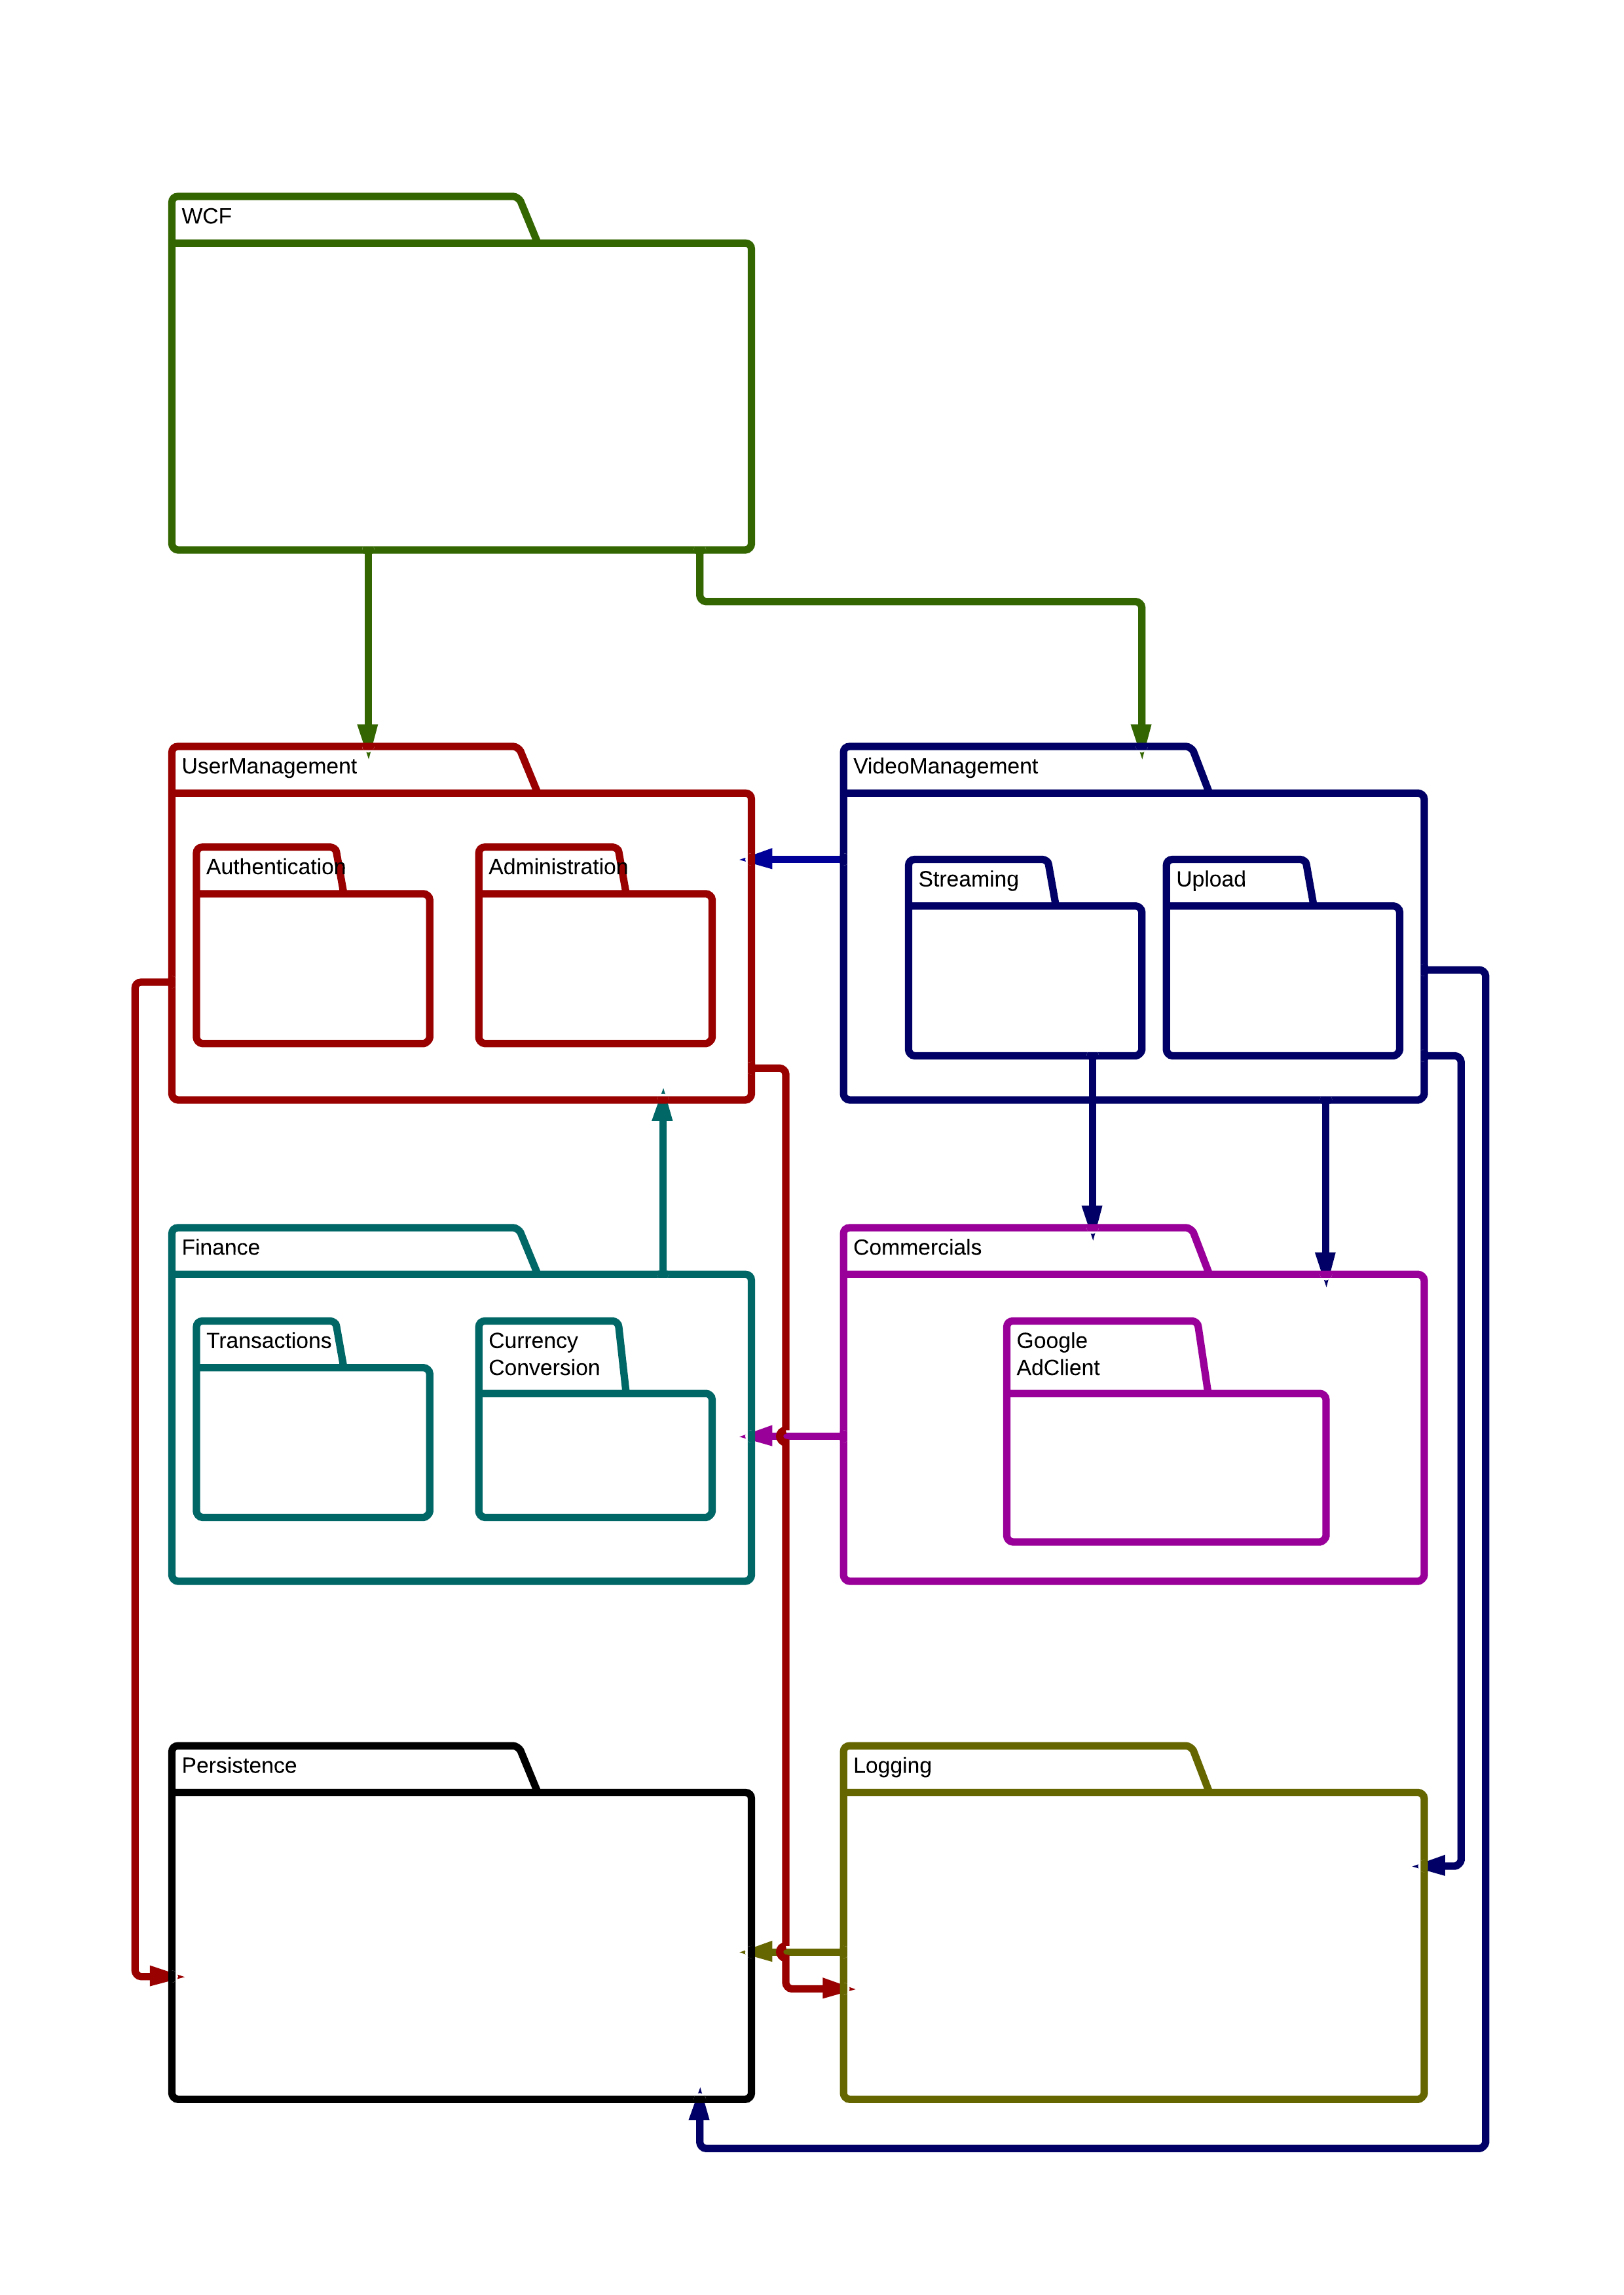
\includegraphics[scale=0.15]{PackageDiagram.png}
\end{center}
\section{Project Management Plan}
